\chapter{Resultados}
\label{chap:result}
A elaboração de cronogramas, e a organização das atividades em pacotes com metas de curto médio e longo prazo contribuiu para que o andamento do projeto ocorresse de forma satisfatória. Os prazos foram mudados  durante o projeto e os atrasos gerados por problemas inesperados conseguiram ser compensados com uma mudança na forma de gerir os integrantes e a inserção de tarefas em paralelo, sendo elas individuais e em subgrupos.


%--------- NEW SECTION ----------------------
\section{Testes unitários}
\label{sec:testu}
Consistem nos testes individuais das ferramentas, tem suma importância para atestar se as ferramentas pré determinadas funcionam de acordo com o esperado.


\subsection{Configuração dos servomotores}
Os primeiros testes realizados no início do desenvolvimento do robô foram a configuração dos servomotores, etapa essencial para a definição de como os motores deveriam trabalhar em conjunto. A configuração se deu utilizando diversos softwares, e após as configurações realizadas, os motores eram analisados para validar se a configuração fora realizada de maneira correta.  O teste foi realizado no período de 22 de junho a 7 de julho pelos componentes: Carlos, Cleber, Davi e Ícaro.

\subsubsection{Utilização do software Mixcell}
O software Mixcell disponível para utilização gratuita na Ros Wiki, possui a funcionalidade de realizar a configuração de parâmetros em motores Dynamixel de diversos modelos, tais como ID dos motores, modos de operação, baudrate para comunicação serial. O software foi utilizado em toda as etapas de testes dos motores, sendo fundamental para determinar o funcionamento de cada um dos motores e para o desenvolvimento e montagem do robô.  

\begin{figure}[h!]												
	\centering												
	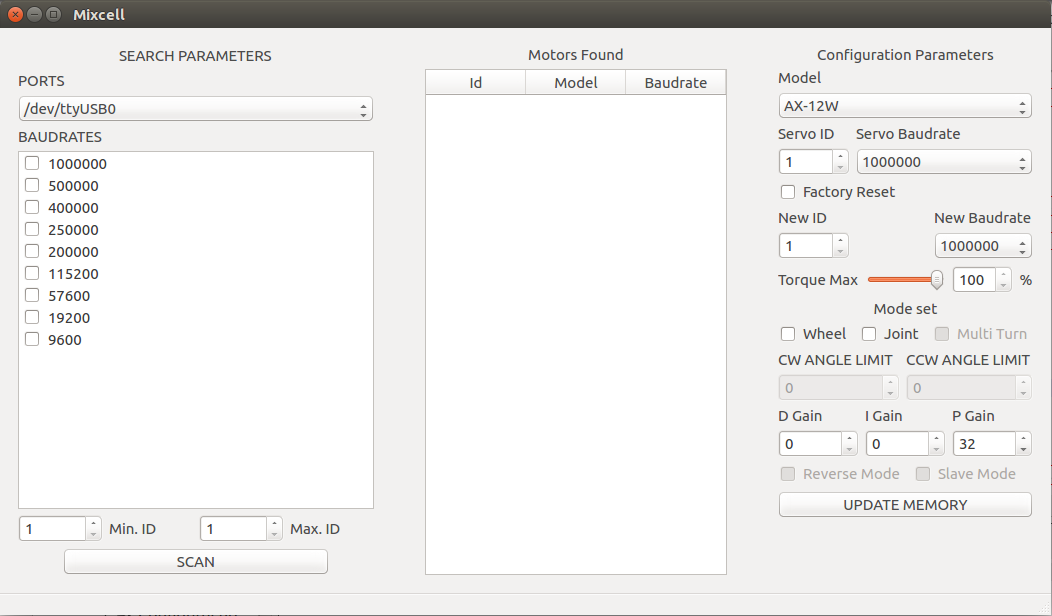
\includegraphics[width=0.8\textwidth]{mixcell.png}				
	\caption{Programa para configuração dos servomotores}		
	\label{img:mixcell}
	\source{Própria}												
\end{figure}		
\subsubsection{Modos Mestre/Escravo}
Durante os testes em modo Mestre/Escravo dos motores Dynamixel, foi observado que mesmo quando dois motores são configurados para trabalharem como mestre/escravo via software, é necessário que se haja a utilização do cabo de sincronização entre os dois motores. Foi constatado durante os testes que o cabo de sincronização transmite a informação de carga para que haja a compensação entre os motores quando trabalham em conjunto. 

\subsubsection{ID, Baud rate e Modos de operação}
Durante toda a fase de testes foram observados parâmetros extremamente importantes para definição e funcionamento dos motores Dynamixel. Os IDs dos motores definem basicamente a sua identificação para as configurações de juntas, associando assim os motores as suas respectivas juntas. 
O baud rate é a taxa de transmissão de dados em bits por segundo entre o computador e os motores. Percebeu-se que durante os testes, para um número grande de motores trabalhando em conjunto, era necessário um valor de baudrate mais elevado para que todos os motores fossem encontrados. 
Os modos de operação dos motores são parâmetros que definem como os mesmos vão se comportar durante a operação, sendo eles os modos junta e roda. No primeiro modo é necessário estabelecer um limite máximo e mínimo para o giro dos motores, além da definição de qual  motor será o mestre ou o escravo durante a operação (caso haja mais de um motor na junta), enquanto que no modo roda o motor irá girar livremente, mudando somente o sentido de giro. 

\subsection{Controle dos servomotores utilizando a biblioteca dynamixel driver}
A biblioteca dynamixel driver foi a utilizada nesse projeto e tal, para fazer a configurações , criar os controladores, possibilitar a integração do motor no sistema ros. Essa biblioteca foi descontinuada na versão utilizada no projeto, o que fez com se mostrassem necessários testes extras. Os testes foram realizado  entre 7 de julho até 21 de julho por Carlos, Cleber, Davi e Ícaro, durante a fase inicial do projeto.

\subsubsection{Controladores de posição}
Foi realizado o teste dos motores de posição para verificar o comportamento dos mesmos. Nas juntas dos braços do robô foi utilizado o modo de controlador de posição, isto é: o motor recebe um comando de posição, que no caso é de 0 a 2PI radianos e assim é possível controlar para  onde o braço irá se mover.
 
O controlador recebe um arquivo de configuração das juntas, especificando os ids e assim pode-se controlar cada um individualmente. Foi realizado o teste em todas as juntas de posição do ELIR.

\subsubsection{Controladores de velocidade}
Os controladores individuais de velocidade tem a função de controlar a velocidade do motor, sem controlar a posição. O motor irá rodar livremente com uma velocidade determinada até que receba um comando para parar. Este controlador foi usado nas rodas das garras que possuem a finalidade de fazer o robô andar sobre a linha. Cada roda fora testada individualmente.

\subsubsection{Controlador de trajetoria}
O controlador de trajetória controller realiza o controle do posicionamento da junta como um todo. Neste controlador é possível controlar diversas juntas diferentes do robô por meio de uma única mensagem no \textit{ROS}, contendo o nome das juntas que deverão ser controladas, as posições desejadas, tempos de execução, velocidades e esforço. Esse controlador se mostrou extremamente importante e eficiente pela sua capacidade de agrupar diversas juntas em um único comando de movimento. 

\subsubsection{Compatibilidade com diferentes protocolos de comunicação}
Há uma limitação na biblioteca dynamixel driver, esta funciona somente para motores com firmware versão 1.0 devido a sua descontinuação. Foi testado para todas as versões contidas nos motores que possuíam e não houveram falhas em encontrar nenhum motor na biblioteca. Entretanto, caso houvesse necessidade de atualizar para versão v2.0, no qual possui uma taxa de baud rate maior e protocolo de comunicação melhorado, haveria a necessidade de parar com o uso a dynamixel driver e utilizar a biblioteca oficial da fabricante, a dynamixel workbench.

\subsection{Controle dos servomotores utilizando a biblioteca dynamixel workbench}
A biblioteca do \textit{ROS} dynamixel workbench  é outro driver para comunicação com os servomotores, recebe suporte e atualizações diretamente da ROBOTIS, sendo o driver de controle padrão do \textit{ROS} para versões superiores a Kinetc. Considerou se utilizar essa ferramenta devido aos problemas de comunicação apresentados pelos motores. Ela oferece suporte para o protocolo de comunicação na versão 2.0, que suporta uma maior baudrate e muda a estrutura de comunicação.

\subsubsection{Controladores de posição}
A biblioteca oferece a opção de criar controladores de posição individuais para cada motor, sem especificar o ID. Não possibilitando uma criação controlador mestre-escravo para as juntas do robô que são atuadas por 2 motores e também a opção de selecionar quais motores da rede seriam transformados em controladores de posição, o arquivo que instancia os controladores só recebe um alcance de IDs que deve buscar na rede, transformando todos os motores nesse alcance em controladores de posição individuais.

\subsubsection{Controladores de velocidade}
Os controladores de velocidade só recebem o ID de dois motores, assim não apresentando um uso trivial, já que o robô necessita de 5 controladores de velocidade diferentes. Foi encontrado um arquivo customizado no repositório da biblioteca, mas mesmo assim não pode ser utilizado em conjunto com controladores de posição.

\subsubsection{Controladores de trajetória}
Os controladores de trajetória esperados para compatibilização com o planejamento de movimento são os padrões oferecidos pela biblioteca embutida do \textit{ROS}, o \verb|ros_control|. Porém a biblioteca não oferece um driver que instancie esses controladores de trajetória, assim não possibilitando a integração dela com o planejamento de movimento.

\subsubsection{Comunicação em rede}
Em comparação com a biblioteca \verb|dynamixel_drivers|, a comunicação em rede dos servomotores utilizando a biblioteca \verb|dynamixel_workbench| é levemente superior. Quando a comunicação apresentava problemas, essa biblioteca se mostrou mais eficiente para encontrar os motores conectados na rede porém não possibilita o funcionamento completo, já que o \textit{MoveIt!} controla o \textit{ROS} por meio dos controladores de trajetória, assim não se mostrando uma opção para resolução dos problemas de comunicação com os motores.
Essa biblioteca oferece suporte para motores com protocolo 1.0 e 2.0 ,possibilitando criar uma rede com motores dos dois tipos, porém apresenta erros caso os motores tenham o mesmo ID, mas não foram feitos testes de controle para motores com dois protocolos diferentes.

\subsection{Placa de Power Management}
A placa de power management é responsável pelo gerenciamento de energia do robô, ela distribui de forma separada a potência para cada parte elétrica ou eletrônica, e pela sua capacidade de monitoramento, pode identificar e atuar sob algum erro na alimentação. Diversos testes foram feitos para garantir que a mesma estivesse trabalhando de maneira correta.

\subsubsection{Gravação e validação do firmware}
A gravação do firmware na placa de Power Management só foi realizada devido a utilização de um botão para conectar dois pinos específicos da placa (-VIN e S2) para que o microcontrolador fosse alimentado, e a conexão da placa em uma porta USB de um computador.
 
Para que fosse possível estabelecer a comunicação entre o computador e a placa, foi necessário configurar as permissões necessárias no Ubuntu. Durante a gravação do firmware fora utilizada uma extensão do VSCode, o PlatformIO, específica para programação com microcontroladores, para realização de debug e gravação do firmware na placa. 

Durante o processo de gravação foi necessário manter o botão pressionado. Após a gravação do firmware na placa, o seu funcionamento fora validado através do uso dos serviços e mensagens gerados no ambiente \textit{ROS}, uma vez que as informações de níveis de corrente e tensão das portas da placa eram publicados nos tópicos específicos. O teste foi coordenado por Ícaro Nascimento no dia 1 de agosto de 2018.

\subsection{Compatibilidade do Robô com o \textit{MoveIt!}}
Testes realizados no período de 24/05 até 26/06, pelos integrantes Cleber Couto e Davi Oliveira. o teste consiste na criação do pacote \textit{MoveIT!}. O \textit{MoveIt!} fornece uma ferramenta de configuração denominada \textit{MoveIt! Setup Assistant}, que gera a maior parte dos arquivos necessários para a compatibilização. 
\begin{figure}[h!]												
	\centering												
	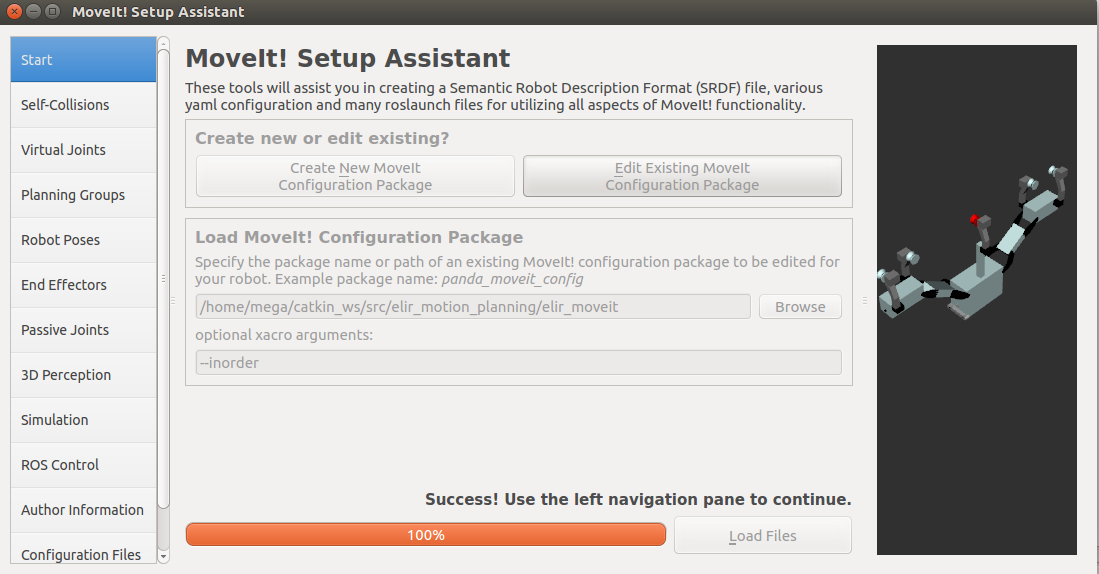
\includegraphics[width=0.8\textwidth]{setup_assistant_elir.png}				
	\caption{Ferramenta para geração de pacote fornecida pelo \textit{MoveIt!}}		
	\label{img:setup_assistant}
	\source{Própria}												
\end{figure}

\subsubsection{Estado de Colisão}
Durante a configuração dos Setup Assistant , o robô apresentava um erro informando que o seu modelo estava em estado de colisão, o que significa que as partes do seu modelo estavam posicionadas erradas e estariam sempre colidindo.

Foi feito um teste removendo todas as partes do robô do arquivo de configuração e checando se a indicação de erro sumia. Com as tentativas se concluiu o problema era o modelo 3D utilizado nas rodas do robô, que gerava a colisão quando se utilizava ele mais de uma vez, a resolução foi a criação de um novo modelo 3D para as rodas, após a substituição o erro sumiu.

\subsubsection{Definição da corrente-cinemática e \textit{end-effector}}
No estudo de cinemática inversa na robótica, corrente cinemática é o nome dado para o conjunto de links e juntas que se vai calcular o movimento, onde o começo dessa corrente é a referência para o cálculo da cinemática e o final da corrente é o end-effector.  No caso do \textit{ELIR}, é necessário se definir duas correntes cinemáticas, já que são dois braços. Com a corrente cinemática definida corretamente ,o \textit{MoveIt!} consegue enviar o comando para movimentar as juntas da corrente simultâneamente.

Ao definir o grupo de controle no Setup Assistant, o usuário escolhe as juntas que irão fazer parte desse grupo, e a corrente cinemática é gerada automaticamente. Foram feitos teste considerando como parte da corrente somente as duas juntas do braço, porém ao analisar outros robôs que já haviam sido configurados, notou-se que sempre se levava em consideração a junta da base do robô para definição do grupo, onde a junta da base é a junta que prende o robô no mundo.

\subsection{Robô de testes \textit{Victory}}
Como o Setup-Assistant oferece diversas opções de configuração, optou-se por desenvolver um modelo de robô mais simples que o \textit{ELIR}, de forma que se pudessem testar os conceitos, e compreender melhor a relação entre as configurações do modelo e os resultados esperados para movimento.
Esse teste foi executado pelos membros Cleber Couto e Davi Oliveira, no período de 6 a 23 de agosto onde esse modelo foi inteiramente escrito pela equipe, tomando como base boas práticas observadas em robôs já compatibilizados com o \textit{MoveIt!}. O \textit{Victory} foi construído como mostra a imagem \ref{img:victory}:

\begin{figure}[h!]												
	\centering												
	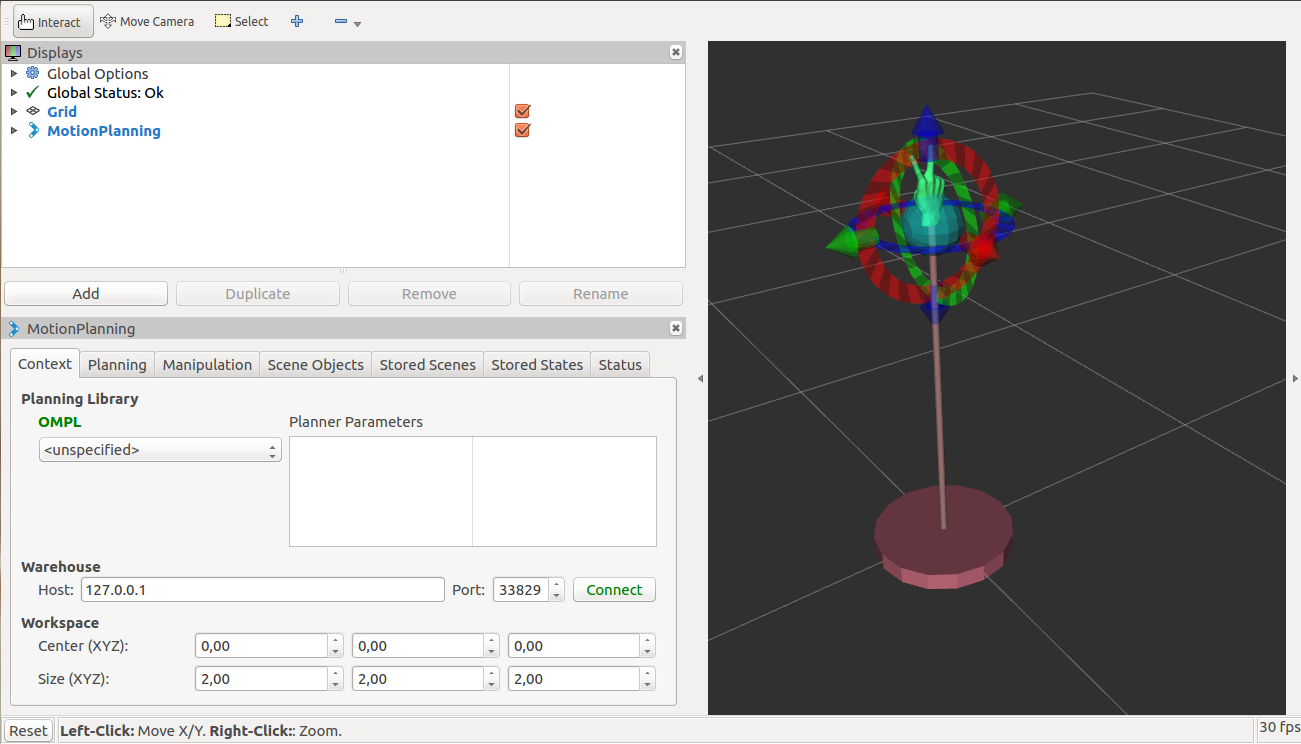
\includegraphics[width=0.8\textwidth]{victory_moveit.png}				
	\caption{Victory Robot na ferramenta de visualização \textit{Rviz}}		
	\label{img:victory}
	\source{Própria}												
\end{figure}

Antes de realizar qualquer modificação na modelagem do robô \textit{ELIR} primeiramente essa modificação foi feita Davictory, assim foram prevenidos quaisquer mudanças desnecessárias e otimizado o tempo devido que o robô customizado ser mais simples. Todos os testes com o planejamento de movimento foram validados também nele.

\subsubsection{Teste com diferentes plugins de cinemática}
Para configurar o pacote do \textit{MoveIT!} de qualquer modelo de robô, é necessário definir qual solucionador de cinemática será utilizado. Como existem variados tipos de robôs com finalidades e conjuntos de movimentos diferentes essa escolha deve ser feita de forma precisa para que o robô em questão realize o movimento de forma eficiente.

Durante a escolha para a cinemática do \textit{ELIR} foi percebido que nenhuma solução se encaixava nas descrições devido ao número reduzido de graus de liberdades (o \textit{ELIR} possui 2 graus de liberdades e os plugins necessitam de no mínimo 3).

A partir de plugins e o \textit{URDF} é possível criar a solução específica para o robô. A fim de achar uma solução que atendesse ao funcionamento do \textit{ELIR}, foram testados no Davictory todos os plugins de cinemática contidos no site oficial do \textit{MoveIT!}. Nenhum plugin obteve sucesso em resolver a cinemática inversa.

%--------- NEW SECTION ----------------------
\section{Testes integrados}
\label{sec:testi}
Após a realização dos testes unitários, validando os conceitos e funcionalidades individualmente, novos testes foram realizados para validação das funcionalidades em conjunto, na etapa de testes unitários.

\subsection{Teste dos limites de giro das juntas}
Este teste realizado por Carlos Alberto e Ícaro Nascimento entre os dias 2 a 24 de Agosto de 2018, teve como objetivo compatibilizar os limites de giro das juntas nos controladores da biblioteca \verb|dynamixel_drivers| com os limites físicos do robô, a fim de evitar colisões. Os limites a princípio vieram do arquivo \textit{URDF} utilizado no \textit{MoveIt!}. Porém, algumas juntas ainda estavam colidindo, então os limites tiveram que ser reajustados manualmente.

\subsection{Integração do \textit{MoveIt! com os controladores do \textit{ROS}}}
Este teste foi feito por Cleber no período de 10 de agosto de 2018 até 11 de setembro de 2018 . Para a compatibilização do MoveIt! com os controladores do \textit{ROS} é necessário que o programa conheça o estado atual do robô e os controladores de trajetória disponíveis, foi necessário desenvolver uma solução que transformasse as informações provenientes dos motores em uma estrutura específica que descreve o estado do robô, provida pelo \textit{ROS}.
 
O mesmo se deu pelo tópico de informação dos motores, porém a informação de posição de cada motor não dá o valor de ângulo de giro, mas sim o valor escrito no registrador do Dynamixel e também não leva em consideração a referência em que cada motor foi configurado, assim sendo necessário uma compensação de referência em código e uma conversão para radianos, assim como a inserção na estrutura padrão do \textit{ROS} para estado atual do robô.

\subsection{Serviço para levantar a garra}
Para realizar a transposição de objetos na linha o robô precisa realizar movimentos específicos. Um desses movimentos se dá em levantar as garras para que as mesmas fiquem livres para fazer a abertura. Esse movimento de levantar foi feito em forma de serviço no \textit{ROS}, no qual basta somente chamar e solicitar a levantamento e abaixamento das garras. O teste foi feito primeiramente no Gazebo e quando ocorreu de forma esperada, foi iniciado o teste no robô físico. A simulação e atuação do teste foi feito pelo integrante Davi Oliveira na data de 7 de novembro de 2018 até 9 de novembro de 2018.

\subsection{Serviço de abrir e fechar as garras}
Foi testado o serviço desenvolvido para realizar a abertura e fechamento das garras, o movimento de abrir é realizado para que o obstáculo passe livremente pelo centro e ao finalizar as garras são fechadas. Observou se que o movimento devia levar em consideração o choque entre as garras, admitindo assim somente um sentido. A resolução se deu por trocar o sinal das coordenadas e observar o o comportamento, assim encontrando a melhor opção. O teste foi feito por Cleber Couto na data de 12 de outubro de 2018.

\subsection{Serviço para levantar haste central na linha}
Para a ultrapassagem de um tipo de obstáculo, a melhor forma encontrada foi de aumentar a distância entre as duas unidades de tração, fazendo com que a haste central se levante, e o obstáculo seja atravessado, foi desenvolvido um serviço para que o robô executasse esse movimento. O teste do serviço fora realizado para funcionamento via simulação em Gazebo. Foi necessário realizar a verificação da posição das juntas para que o robô estivesse na posição esticada e a após este procedimento um ajuste foi realizado. A simulação foi realizada pelo integrante Ícaro Nascimento no dia 16 de novembro de 2018.

\begin{figure}[h!]												
	\centering												
	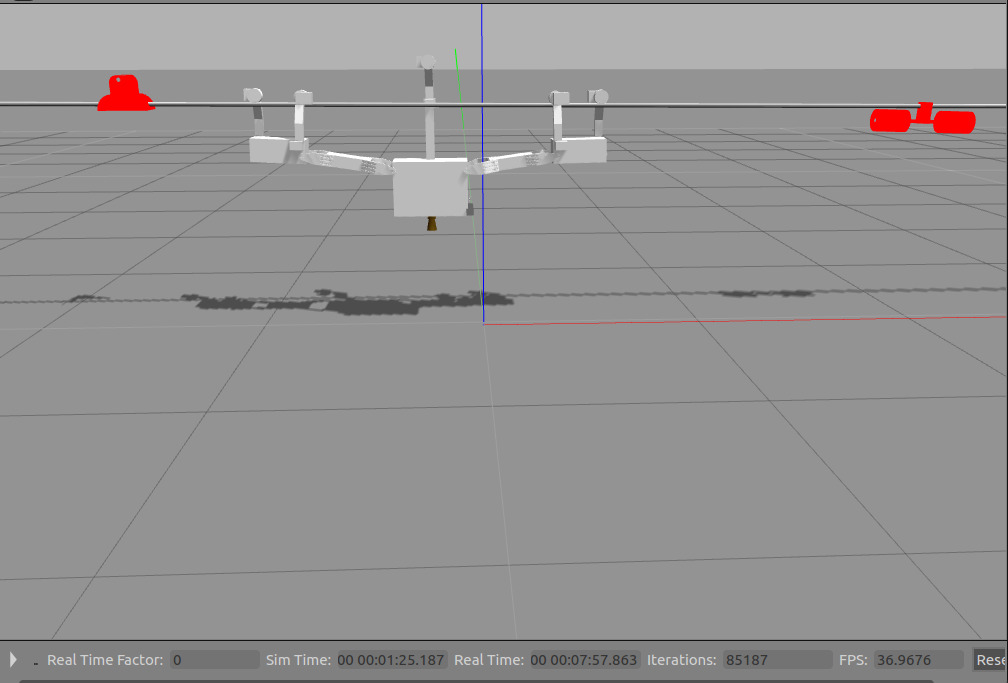
\includegraphics[width=0.6\textwidth]{robot_stretch.png}				
	\caption{\textit{ELIR} realizando o movimento na simulação}		
	\label{img:robot_stretch}
	\source{Própria}												
\end{figure}
  
\subsection{Robô na linha sem alimentação}
Quando toda a estrutura mecânica do robô estava completamente montada, o mesmo foi colocado sobre uma linha de testes localizada no estacionamento do Senai  Cimatec. O teste foi coordenado por Cléber, Marco e Ícaro no dia 10 de setembro de 2018, e consistiu em posicionar o robô na linha de transmissão para verificar o alinhamento das garras e a distribuição do peso. Foi observado que havia um desalinhamento entre as rodas das garras dos motores. Após a observação deste erro as garras foram reposicionadas durante uma nova montagem do robô, resolvendo o problema do desalinhamento.

\subsection{Robô na linha utilizando alimentação alternativa}
No primeiro teste na linha de transmissão, que ocorreu no dia 19 de outubro de 2018, foi montado um setup com uma bateria automotiva 12V - 70Ah para alimentar todos os componentes do robô. A NUC foi alimentada com sua fonte conectada a um inversor que por sua vez estava ligado à bateria. Nesse teste não houve sucesso na comunicação com os motores, a bateria nesse momento fornecia 12,17V e era a única modificação em relação aos testes no laboratório. Com a fonte de bancada, nenhum problema de comunicação aconteceu. O teste foi conduzido por Carlos, Cleber, Davi e Ícaro.

\subsection{Alimentação do sistema utilizando \textit{Nobreak}}
Para contornar o problema encontrado no primeiro teste na linha de transmissão, a alimentação seria fornecida pela mesma fonte de bancada dos testes unitários e esta seria ligada a um nobreak. Com o nobreak ligado na tomada a fonte foi ajustada em 14V, no momento em que a tomada era desconectada, a fonte passava a fornecer 10V variando por volta de 200mV. Teste realizado no dia 22 de outubro por Carlos.

\subsection{Teleoperação para movimentação na linha}
Para conseguir mover o robô na linha e observar o seu comportamento, era necessário desenvolver uma forma de o operador controlar a velocidade das rodas de forma intuitiva. O teste foi conduzido por Cleber e Carlos, no período de: 12 a 24 de outubro.O \textit{ROS} fornece um driver de teleoperação via teclado, foi criado um nó que faz a interface desse pacote com os controladores do robô, possibilitando assim testar o deslocamento horizontal na linha. Foi observado que os motores não param de girar assim que a tecla para de ser pressionada, devido a velocidade que o nó do teclado atualiza os comandos.

\subsection{Alimentação de todos os motores pela placa de \textit{Power Management}}
Após a validação do funcionamento da placa de gerenciamento de energia, foi necessário verificar se o seu fornecimento de energia seria suficiente para alimentar toda a rede de motores para que pudessem operar em conjunto. O teste conduzido por Davi e Ícaro no dia 31 de outubro, consistiu em conectar todos os três hubs dos motores nas portas da Power Management, monitorando o seu funcionamento. Nos testes iniciais fora percebido que os picos de corrente dos motores faziam com que a alimentação nas portas fossem interrompidas. Tendo em vista a ocorrência desse problema foi necessário ajustar os limites de corrente via serviço em \textit{ROS} da placa para que a alimentação não fosse interrompida durante a operação.

\subsection{Comunicação dos motores em rede}
Os dynamixel se comunicam serialmente por meio do padrão físico RS485, que possui uma boa imunidade a ruídos, distância de comunicação e número de receptores maiores do que foi usado. O teste constituiu colocar em paralelo todos os motores por meio dos hubs construídos e assim verificar se o \textit{ROS} o encontram. Foi feita a instalação dos motores na estrutura do robô, realizando as conexões com os cabos de alimentação e comunicação padrão junto com os HUBs desenvolvidos para cada grupo de motores. O driver para os motores fornece a função de busca em rede, o que foi suficiente nesse teste para garantir que os motores estavam se comunicando.

Durante o teste dos motores em rede foi encontrado o problema de achar apenas alguns motores de forma aleatória,  dos 18 conectados. Foi feita uma série de testes em relação ao firmware para verificar se o problema era na comunicação. A troca, upgrade, downgrade e restauração foram feitos utilizando o software \textit{ROBOPLUS} da própria fabricante dos motores. Os testes foram feitos por Davi Oliveira e Carlos Alberto nos dias 29 de setembro de 2018 até 5 de outubro de 2018.

\subsection{Restauração para \textit{firmware} padrão de fábrica}
O firmware de cada motor foi restaurado para o padrão de fábrica e realizando a busca na rede individual. Os motores estavam funcionando porém ao serem conectados todos ao mesmo tempo, o erro de comunicação persistia.

\subsection{Compatibilização das versões de \textit{firmware}}
A partir da busca de motores que sofriam problemas parecidos, foi encontrado fórum oficial da \textit{Robotis}, que a versão do mais estável era a versão v1.0 -36 para os motores que foram utilizados.
Foi verificado que a maioria dos motores estavam na versão v1.0 - 36 e somentes alguns estavam na v1.0 - 37. Foi feita a troca do que constam v1.0 -37 para v1.0 -36 e ainda assim o problema se mostrou consistente.

\subsection{Atualização para versão de \textit{firmware} v2.0}
 Foi testado a troca de firmware para versão v2.0 no qual possui evolução no protocolo de comunicação assim como uma maior baudrate, houve melhora em relação à quantidade de motores encontrados mas ainda assim o problema se mostrou ativo.

\subsection{Troca dos motores danificados}
Como os testes anteriores não apresentaram solução, foi realizado um teste onde os motores eram inseridos na rede de um a um, onde a comunicação era verificada. Quando a comunicação começava a apresentar falhas, esse motor era retirado da rede, assim foram encontrados 2 motores que inseriam esse erro de comunicação na linha. Os motores funcionavam indivualmente e quando conectados com uma pequena quantidade de motores. O problema da falta de comunicação foi sanado após a troca dos motores defeituosos.

%--------- NEW SECTION ----------------------
\section{Avaliação da prontidão tecnológica}
\label{sec:trl}
Uma das ferramentas conhecidas para a avaliação de tecnologias é a matriz TRL desenvolvida pela NASA\footnote{National Aeronautics and Space Administration} e que permitir definir o nível de maturidade de uma tecnologia. Entende-se que a tecnologia é definida como a aplicação prática do conhecimento para criar a capacidade de fazer algo inteiramente novo de forma inteiramente nova, o que difere da pesquisa científica que engloba a descoberta de um novo conhecimento da qual a tecnologia é derivada.

A importância do uso dessa avaliação, encontra seu respaldo no quesito de nortear o desenvolvimento do projeto na minimização dos gastos oriundos de uma orçamentação e também no conhecimento das tecnologias plausíveis para o desenvolvimento da solução requerida.

%\section{A matriz BTRL}
Todo projeto foi acompanhado por uma cadência de avaliações ao longo das fases do projeto. Estas avaliações seguem as diretrizes da ISO 16290, a qual estabelece níveis do quanto uma tecnologia está desenvolvida, tomando como base este procedimento e levando em consideração as avaliações de risco para um projeto de R\&D\footnote{Research and Development}, criou-se o BTRL\footnote{BIR Technology Readiness Level}. 

% Please add the following required packages to your document preamble:
% \usepackage[table,xcdraw]{xcolor}
% If you use beamer only pass "xcolor=table" option, i.e. \documentclass[xcolor=table]{beamer}
%\begin{sidewaystable*}
\begin{table}[h]
\centering
\caption{Matriz do Nível de Prontidão Tecnológia do Senai Cimatec.}
\begin{adjustbox}{width=1\textwidth}
\label{tabela:BTRL}
\begin{tabular}{lc|p{1.5cm} p{1.5cm} p{1.5cm} p{1.5cm}}
\cline{1-2}
\multicolumn{2}{|l|}{\cellcolor[HTML]{000000}{\color[HTML]{FFFFFF} \textbf{NÍVEL DA PRONTIDÃO TECNOLÓGICA}}} &  &  &  &  \\ \cline{1-2}
\multicolumn{1}{|l|}{\textbf{perspectiva}} & \textbf{nível} &  &  &  &  \\ \hline
\multicolumn{1}{|l|}{\textit{sistema aprovado}} & \textit{9} & \multicolumn{1}{c|}{\cellcolor[HTML]{F56B00}L2} & \multicolumn{1}{c|}{\cellcolor[HTML]{F8FF00}{\color[HTML]{FFFFFF} L3}} & \multicolumn{1}{c|}{\cellcolor[HTML]{009901}{\color[HTML]{FFFFFF} L4}} & \multicolumn{1}{c|}{\cellcolor[HTML]{009901}{\color[HTML]{FFFFFF} L4}} \\ \hline
\multicolumn{1}{|l|}{\textit{sistema qualificado}} & \textit{8} & \multicolumn{1}{c|}{\cellcolor[HTML]{F56B00}L2} & \multicolumn{1}{c|}{\cellcolor[HTML]{F8FF00}{\color[HTML]{FFFFFF} L3}} & \multicolumn{1}{c|}{\cellcolor[HTML]{009901}{\color[HTML]{FFFFFF} L4}} & \multicolumn{1}{c|}{\cellcolor[HTML]{009901}{\color[HTML]{FFFFFF} L4}} \\ \hline
\multicolumn{1}{|l|}{\textit{protótipo testado em campo operacional}} & \textit{7} & \multicolumn{1}{c|}{\cellcolor[HTML]{F56B00}L2} & \multicolumn{1}{c|}{\cellcolor[HTML]{F8FF00}{\color[HTML]{FFFFFF} L3}} & \multicolumn{1}{c|}{\cellcolor[HTML]{009901}{\color[HTML]{FFFFFF} L4}} & \multicolumn{1}{c|}{\cellcolor[HTML]{009901}{\color[HTML]{FFFFFF} L4}} \\ \hline
\multicolumn{1}{|l|}{\textit{protótipo testado em campo relevante}} & \textit{6} & \multicolumn{1}{c|}{\cellcolor[HTML]{9A0000}{\color[HTML]{FFFFFF} L1}} & \multicolumn{1}{c|}{\cellcolor[HTML]{F56B00}L2} & \multicolumn{1}{c|}{\cellcolor[HTML]{F8FF00}{\color[HTML]{FFFFFF} L3}} & \multicolumn{1}{c|}{\cellcolor[HTML]{009901}{\color[HTML]{FFFFFF} L4}} \\ \hline
\multicolumn{1}{|l|}{\textit{funcionalidades testadas em campo relevante}} & \textit{5} & \multicolumn{1}{c|}{\cellcolor[HTML]{9A0000}{\color[HTML]{FFFFFF} L1}} & \multicolumn{1}{c|}{\cellcolor[HTML]{F56B00}L2} & \multicolumn{1}{c|}{\cellcolor[HTML]{F8FF00}{\color[HTML]{FFFFFF} L3}} & \multicolumn{1}{c|}{\cellcolor[HTML]{009901}{\color[HTML]{FFFFFF} L4}} \\ \hline
\multicolumn{1}{|l|}{\textit{funcionalidades testadas em laboratório}} & \textit{4} & \multicolumn{1}{c|}{\cellcolor[HTML]{9A0000}{\color[HTML]{FFFFFF} L1}} & \multicolumn{1}{c|}{\cellcolor[HTML]{F56B00}L2} & \multicolumn{1}{c|}{\cellcolor[HTML]{F56B00}L2} & \multicolumn{1}{c|}{\cellcolor[HTML]{F8FF00}{\color[HTML]{FFFFFF} L3}} \\ \hline
\multicolumn{1}{|l|}{\textit{conceito aprovado}} & \textit{3} & \multicolumn{1}{c|}{\cellcolor[HTML]{9A0000}{\color[HTML]{FFFFFF} L1}} & \multicolumn{1}{c|}{\cellcolor[HTML]{9A0000}{\color[HTML]{FFFFFF} L1}} & \multicolumn{1}{c|}{\cellcolor[HTML]{F56B00}L2} & \multicolumn{1}{c|}{\cellcolor[HTML]{F56B00}L2} \\ \hline
\multicolumn{1}{|l|}{\textit{conceito formulado}} & \textit{2} & \multicolumn{1}{c|}{\cellcolor[HTML]{9A0000}{\color[HTML]{FFFFFF} L1}} & \multicolumn{1}{c|}{\cellcolor[HTML]{9A0000}{\color[HTML]{FFFFFF} L1}} & \multicolumn{1}{c|}{\cellcolor[HTML]{9A0000}{\color[HTML]{FFFFFF} L1}} & \multicolumn{1}{c|}{\cellcolor[HTML]{F56B00}L2} \\ \hline
\multicolumn{1}{|l|}{\textit{princípios básicos aprovados}} & \textit{1} & \multicolumn{1}{c|}{\cellcolor[HTML]{9A0000}{\color[HTML]{FFFFFF} L1}} & \multicolumn{1}{c|}{\cellcolor[HTML]{9A0000}{\color[HTML]{FFFFFF} L1}} & \multicolumn{1}{c|}{\cellcolor[HTML]{9A0000}{\color[HTML]{FFFFFF} L1}} & \multicolumn{1}{c|}{\cellcolor[HTML]{9A0000}{\color[HTML]{FFFFFF} L1}} \\ \hline
 &  & \multicolumn{1}{c|}{\textbf{\begin{tabular}[c]{@{}c@{}}muito \\ alto\end{tabular}}} & \multicolumn{1}{c|}{\textbf{alto}} & \multicolumn{1}{c|}{\textbf{médio}} & \multicolumn{1}{c|}{\textbf{baixo}} \\ \cline{3-6} 
 &  & \multicolumn{4}{c|}{\cellcolor[HTML]{000000}{\color[HTML]{FFFFFF} \textbf{CATEGORIZAÇÃO DO RISCO TÉCNICO}}} \\ \cline{3-6} 
\end{tabular}
\end{adjustbox}
\end{table}	
%\end{sidewaystable*}

O BTRL é o índice destas duas variáveis: TRL e Riscos. A matriz apresenta através da Tabela \ref{tabela:BTRL} de forma clara a relação entre estes dois critérios, estabelecendo desta forma 4 níveis:
\begin{itemize}
	\item L1 - desenvolvimento significativo requerido.
	\item L2 - requer mais desenvolvimento da tecnologia antes de prosseguir para a próxima fase do projeto.
	\item L3 - requer alguns desenvolvimento adicional na tecnologia.
	\item L4 - pronto para uso tanto do protótipo para as fases seguintes, como para o uso do produto em campo.
\end{itemize}
No entanto, deve-se estabelecer critérios para os níveis de riscos atingidos. Onde foi utilizado para a avaliação destes riscos outras duas variáveis importantes: o nível de confiabilidade do sistema e o nível do protótipo/sistema que se está sendo desenvolvido (conforme Tabela \ref{tabela:TRC}).

% Please add the following required packages to your document preamble:
% \usepackage[table,xcdraw]{xcolor}
% If you use beamer only pass "xcolor=table" option, i.e. \documentclass[xcolor=table]{beamer}
\begin{table}[h]
\centering
\caption{Categorização dos Riscos Técnicos - TRC.}
\begin{adjustbox}{width=1\textwidth}
\label{tabela:TRC}
\begin{tabular}{lc|p{2.5cm}p{2.5cm}p{2.5cm}p{2.5cm}}
\cline{1-2}
\multicolumn{2}{|l|}{\cellcolor[HTML]{000000}{\color[HTML]{FFFFFF} \textbf{PROTÓTIPO}}} &  &  &  &  \\ \hline
\multicolumn{1}{|l|}{tecnologia aprovada} & 4 & \multicolumn{1}{c|}{\cellcolor[HTML]{F56B00}{\color[HTML]{FFFFFF} B}} & \multicolumn{1}{c|}{\cellcolor[HTML]{F8FF00}C} & \multicolumn{1}{c|}{\cellcolor[HTML]{009901}{\color[HTML]{FFFFFF} D}} & \multicolumn{1}{c|}{\cellcolor[HTML]{009901}{\color[HTML]{FFFFFF} D}} \\ \hline
\multicolumn{1}{|l|}{pequenas modificações} & 3 & \multicolumn{1}{c|}{\cellcolor[HTML]{F56B00}{\color[HTML]{FFFFFF} B}} & \multicolumn{1}{c|}{\cellcolor[HTML]{F8FF00}C} & \multicolumn{1}{c|}{\cellcolor[HTML]{F8FF00}C} & \multicolumn{1}{c|}{\cellcolor[HTML]{009901}{\color[HTML]{FFFFFF} D}} \\ \hline
\multicolumn{1}{|l|}{grandes modificações} & 2 & \multicolumn{1}{c|}{\cellcolor[HTML]{9A0000}{\color[HTML]{FFFFFF} A}} & \multicolumn{1}{c|}{\cellcolor[HTML]{F56B00}{\color[HTML]{FFFFFF} B}} & \multicolumn{1}{c|}{\cellcolor[HTML]{F8FF00}C} & \multicolumn{1}{c|}{\cellcolor[HTML]{F8FF00}C} \\ \hline
\multicolumn{1}{|l|}{novo design conceitual} & 1 & \multicolumn{1}{c|}{\cellcolor[HTML]{9A0000}{\color[HTML]{FFFFFF} A}} & \multicolumn{1}{c|}{\cellcolor[HTML]{9A0000}{\color[HTML]{FFFFFF} A}} & \multicolumn{1}{c|}{\cellcolor[HTML]{F56B00}{\color[HTML]{FFFFFF} B}} & \multicolumn{1}{c|}{\cellcolor[HTML]{F56B00}{\color[HTML]{FFFFFF} B}} \\ \hline
 &  & \multicolumn{1}{p{2.5cm}|}{\footnotesize{melhorias na tecnologia são requeridas}} & \multicolumn{1}{p{2.5cm}|}{\footnotesize{melhorias no design são requeridas}} & \multicolumn{1}{p{2.5cm}|}{\footnotesize{pequenas melhorias são requeridas}} & \multicolumn{1}{p{2.5cm}|}{\footnotesize{não há necessidade de melhorias}} \\ \cline{3-6} 
 &  & \multicolumn{4}{c|}{\cellcolor[HTML]{000000}{\color[HTML]{FFFFFF} \textbf{CONFIABILIDADE}}} \\ \cline{3-6} 
\end{tabular}
\end{adjustbox}
\end{table}

A avaliação dos riscos técnicos (TRC) é categorizada em 4 níveis:
\begin{itemize}
	\item A - risco muito alto
	\item B - risco alto
	\item C - risco médio
	\item D - risco baixo
\end{itemize}

Para os projetos em robótica, será sempre avaliado o protótipo/sistema no final de cada fase do desenvolvimento. Neste caso específico do projeto de Direção Assistida, está sendo avaliado o sistema na fase Conceitual.

\subsection{Avaliação do BTRL para o sistema robótico em desenvolvimento}
De forma a sistematizar a avaliação dos subsistemas, em desenvolvimento para a avaliação do nível de prontidão tecnológica nesta fase do projeto foi tomado a estrutura da arquitetura geral apresentada no início do capítulo \ref{ch:arqg}.
Desta forma obteve-se a seguinte avaliação, conforme apresentada na Tabela \ref{tabela:TRL_FC}.

% Please add the following required packages to your document preamble:
% \usepackage[table,xcdraw]{xcolor}
% If you use beamer only pass "xcolor=table" option, i.e. \documentclass[xcolor=table]{beamer}
\begin{table}[h]
%\scalefont{0.8}
\centering
\caption{Avaliação da Prontidão Tecnológica - Fase Design.}
\label{tabela:TRL_FC}
\begin{tabular}{llccccl}
\rowcolor[HTML]{000000} 
\multicolumn{7}{l}{\cellcolor[HTML]{000000}{\color[HTML]{FFFFFF} FASE DESIGN}} \\
\rowcolor[HTML]{EFEFEF} 
\textbf{subsistemas} 		& \textbf{componentes} 				& RL & PL & TRC & TRL & BRTL\\ \hline
sensoriamento				& gps								& 4	 & 4  & 4	& 9	  & \cellcolor[HTML]{009901}\\ \hline
sensoriamento				& imu								& 4	 & 4  & 4	& 9	  & \cellcolor[HTML]{009901}\\ \hline
sensoriamento				& rgb cam							& 4	 & 4  & 4	& 9	  & \cellcolor[HTML]{009901}\\ \hline
sensoriamento				& vnir cam							& 3	 & 3  & 3	& 8	  & \cellcolor[HTML]{009901}\\ \hline
sensoriamento				& swir cam							& 3	 & 3  & 3	& 8	  & \cellcolor[HTML]{009901}\\ \hline
sensoriamento				& lidar								& 4	 & 4  & 4	& 9	  & \cellcolor[HTML]{009901}\\ \hline
sistema de processamento	    & dau								& 4	 & 4  & 4	& 9	  & \cellcolor[HTML]{009901}\\ \hline
sistema de processamento 	& controlador XY						& 3	 & 4  & 4	& 9	  & \cellcolor[HTML]{009901}\\ \hline
sistema de processamento 	& unidade de rotação					& 3	 & 4  & 4	& 9	  & \cellcolor[HTML]{009901}\\ \hline
sistema de processamento 	& switch								& 4	 & 4  & 4	& 9	  & \cellcolor[HTML]{009901}\\ \hline
sistema de processamento 	& NUC								& 4	 & 4  & 4	& 9	  & \cellcolor[HTML]{009901}\\ \hline
sistem de potência			& baterias							& 4	 & 4  & 4	& 9	  & \cellcolor[HTML]{009901}\\ \hline
sistem de potência			& fonte de alimentação				& 4	 & 4  & 4	& 9	  & \cellcolor[HTML]{009901}\\ \hline
sistem de potência			& no break							& 4	 & 4  & 4	& 9   & \cellcolor[HTML]{009901}\\ \hline
estrutura mecânica			& carenagem							& 4	 & 4  & 4	& 9	  & \cellcolor[HTML]{009901}\\ \hline
estrutura mecânica			& suporte dos sensores				& 4	 & 4  & 4	& 9	  & \cellcolor[HTML]{009901}\\ \hline
estrutura mecânica			& perfis de alumínio					& 4	 & 4  & 4	& 9	  & \cellcolor[HTML]{009901}\\ \hline
estrutura mecânica			& rodas								& 4	 & 4  & 4	& 9	  & \cellcolor[HTML]{009901}\\ \hline
interface					& base de controle					& 4	 & 4  & 4	& 9	  & \cellcolor[HTML]{009901}\\ \hline
interface					& display							& 4	 & 4  & 4	& 9	  & \cellcolor[HTML]{009901}\\ \hline
funcinalidades				& aquisição							& 3	 & 3  & 3	& 5	  & \cellcolor[HTML]{F8FF00}\\ \hline
funcinalidades				& calibração							& 2	 & 2  & 2	& 4	  & \cellcolor[HTML]{F56B00}\\ \hline
funcinalidades				& checking							& 2	 & 2  & 2	& 4	  & \cellcolor[HTML]{F56B00}\\ \hline
funcinalidades				& localização						& 2	 & 3  & 3	& 5	  & \cellcolor[HTML]{F8FF00}\\ \hline
funcinalidades				& navegação							& 2	 & 3  & 3	& 5	  & \cellcolor[HTML]{F8FF00}\\ \hline
funcinalidades				& escaneamento						& 2	 & 2  & 2	& 4	  & \cellcolor[HTML]{F56B00}\\ \hline
funcinalidades				& gestão de dados					& 3	 & 3  & 3	& 4	  & \cellcolor[HTML]{F56B00}\\ \hline
funcinalidades				& gestão de log						& 3	 & 3  & 3   & 4	  & \cellcolor[HTML]{F56B00}\\ \hline
funcinalidades				& interface de operação				& 2	 & 2  & 2	& 4	  & \cellcolor[HTML]{F56B00}\\ \hline
funcinalidades				& interface de pós-processamento		& 2	 & 2  & 2	& 2	  & \cellcolor[HTML]{9A0000}\\ \hline
funcinalidades				& pós-processamento					& 2	 & 2  & 2	& 3	  & \cellcolor[HTML]{9A0000}\\ \hline
\end{tabular}
\end{table}

%Diante disso, faz-se os seguintes comentários:
%\begin{itemize}
%	\item \textbf{VNIR cam}: o conjunto de câmeras hiperespectrais foram testadas em laboratório, quanto a sua operação e funcionamento, as mesmas apresentaram um bom desempenho mas precisam ser integradas ao sistema; seu desempenho em ambiente externo mostrou-se adequado.
%	\item \textbf{SWIR cam}: o conjunto de câmeras hiperespectrais foram testadas em laboratório, quanto a sua operação e funcionamento, as mesmas apresentaram um bom desempenho mas precisam ser integradas ao sistema; seu desempenho em ambiente externo mostrou-se adequado.
%	\item \textbf{aquisição}: esta funcionalidade testada e com dados disponibilizados para testes e consultas.
%	\item \textbf{calibração}: a funcionalidade apresenta em grande parte a integração com os sensores, testes precisam ser realizados para uma melhor otimização.
%	\item \textbf{checking}: funcionalidade isolada no início do desenvolvimento, aumentar atenção para uma aplicação mais profunda.
%	\item \textbf{localização}: intermitência no uso, novas técnicas precisam ser testadas para finalizar o desenvolvimento.
%	\item \textbf{navegação}: funcionalidade em adaptação pela falta da plataforma móvel.
%	\item \textbf{escaneamento}: testes elaborados em laboratório apresentaram uma boa eficiência, precisa ser testado em ambiente relevante.
%	\item \textbf{gestão de dados}: funcionalidade desenvolvida sob o framework ROS, necessita maior entendimento entre a troca de informações com o sistema operacional Windows.
%	\item \textbf{gestão de log}: algoritmo em otimização, muito da funcionalidade já testada em outros projetos.
%	\item \textbf{interface de operação}: apresenta-se de forma simplificada e útil para o contexto de prototipagem.
%	\item \textbf{interface de pós-processamento}: necessita desenvolver, a ideia ainda esta baseada em um \textit{draft}.
%	\item \textbf{pós-processamento}: funcionalidade ainda não testada, porém apresenta consistência na elaboração do algoritmo.
%%	
%\end{itemize}

Tendo como base do desenvolvimento os requisitos técnicos levantados, deve-se também observar os comentários levantados pela avaliação do BTRL e potencializar o desenvolvimento para atingir o nível 4 ou 3 do BTRL dependendo da tecnologia envolvida; acredita-se que nestes níveis o protótipo poderá ser considerado adequado para o nível de TRL 5/6 estabelecido como objetivo pela direção do projeto.

%--------- NEW SECTION ----------------------
\section{Trabalhos futuros}
\label{sec:trabfut}
A implementação de um robô para inspeção de linha, faz possível que sejam implementadas diferentes tipos de tecnologias, já que a sua estrutura pode ser projetada para receber uma série de implementações. Um drone por exemplo, consegue realizar uma manutenção visual efetiva, sem muito gasto energético, mas seu tamanho reduzido faz com que algumas tecnologias não consigam ser implantadas.

Os resultados dos testes possibilitam o início de novos estudos e mostra comportamentos específicos de cada componente que tem que ser levados em consideração. Os servomotores apresentaram um melhor desempenho quando alimentados com 14.4V, conseguindo realizar movimentos que necessitavam de mais torque de forma efetiva, enquanto com 12V o movimento não acontecia de forma consistente. Hoje a ROBOTIS desenvolve modelos de servomotores que possuem um torque máximo muito elevado, assim se torna viável a troca dos motores nas juntas que realizam mais esforço, assim como o estudo para aumento da tensão de alimentação ou um estudo dirigido para encontrar o melhor valor da curva torque e tensão de alimentação.

O \textit{MoveIt}! possibilita a integração com ferramentas de visualização, assim tornando viável a futura implementação de um sistema de controle baseado em percepção 3D e odometria visual. O uso de algoritmos de detecção de obstáculos precisos, torna possível a ultrapassagem automática de obstáculos, sendo possível inserir o obstáculo no ambiente do robô e realizar o desvio automaticamente.







